\documentclass[a4paper,12pt]{scrartcl}
\usepackage[utf8]{inputenc}
\usepackage[UKenglish]{isodate}
\usepackage{csquotes}
\usepackage{graphicx}
\usepackage{wrapfig}
\usepackage{enumitem}
\usepackage{pdflscape}
\usepackage[toc,page]{appendix}
\usepackage{geometry}
\usepackage{hyperref}
\usepackage{cleveref}
\usepackage{listings}
\usepackage{csvsimple}
\usepackage{booktabs}
\usepackage{longtable}
\usepackage{caption}
\usepackage{subcaption}
\usepackage[colorinlistoftodos]{todonotes}
\usepackage[british]{babel}
\usepackage{float}
%\usepackage[margin=1in]{geometry}
\usepackage{listings}
\usepackage{color}
 
\definecolor{codegreen}{rgb}{0,0.6,0}
\definecolor{codegray}{rgb}{0.5,0.5,0.5}
\definecolor{codepurple}{rgb}{0.58,0,0.82}
\definecolor{backcolour}{rgb}{0.95,0.95,0.92}
 
\lstdefinestyle{mystyle}{
	language=PHP,
    backgroundcolor=\color{backcolour},   
    commentstyle=\color{codegray},
    keywordstyle=\color{magenta},
    numberstyle=\tiny\color{codegray},
    stringstyle=\color{codegreen},
    basicstyle=\footnotesize,
    breakatwhitespace=false,         
    breaklines=true,                 
    captionpos=b,                    
    keepspaces=true,                 
    numbers=left,                    
    numbersep=5pt,                  
    showspaces=false,                
    showstringspaces=false,
    showtabs=false,                  
    tabsize=3,
    morekeywords={ new, __halt_compiler, abstract, and, array, as, break, callable, case, catch, class, clone, const, continue, declare, default, die, do, echo, else, elseif, empty, enddeclare, endfor, endforeach, endif, endswitch, endwhile, eval, exit, extends, final, for, foreach, function, global, goto, if, implements, include, include_once, instanceof, insteadof, interface, isset, list, namespace, new, or, print, private, protected, public, require, require_once, return, static, switch, throw, trait, try, unset, use, var, while, xor}
}

\lstset{language=Java,
  showspaces=false,
  showtabs=false,
  breaklines=true,
  showstringspaces=false,
  breakatwhitespace=true,
  commentstyle=\color{pgreen},
  keywordstyle=\color{pblue},
  stringstyle=\color{pred},
  basicstyle=\ttfamily,
  moredelim=[il][\textcolor{pgrey}]{$$},
  moredelim=[is][\textcolor{pgrey}]{\%\%}{\%\%}
}
 
\lstset{style=mystyle}

\graphicspath{ {images/} }
\usepackage[
	backend=biber,
	style=ieee,
	]{biblatex}

\addbibresource{references.bib}

\title{829H1 Real-Time Embedded Systems Exercise 5}
\author{Candidate No: 105936}
\date{\today}

\begin{document}
	
	\begin{titlepage}
		\maketitle
	\end{titlepage}
	
	\tableofcontents
	\newpage
	
	\section{Introduction}
	{
		This report focuses on using Ethernet communications on the board and shows the work completed during the laboratory sessions and what was learnt. Code listings for some of the created programs can be found in \cref{Appendix:start}.
	}
	
	\section{Experiments}
	{
		\subsection{Connect 2 mbed boards via Ethernet}
		{
			\subsubsection{Exercise 1}{
				This was completed using the code provided however did not work at the first attempt this was due to a faulty board. Once the board was replaced it worked as expected. \Cref{img:ex1-client} and \Cref{img:ex1-server} shows the outputs from the application once the new board was substituted.
				\begin{figure}
					\centering
					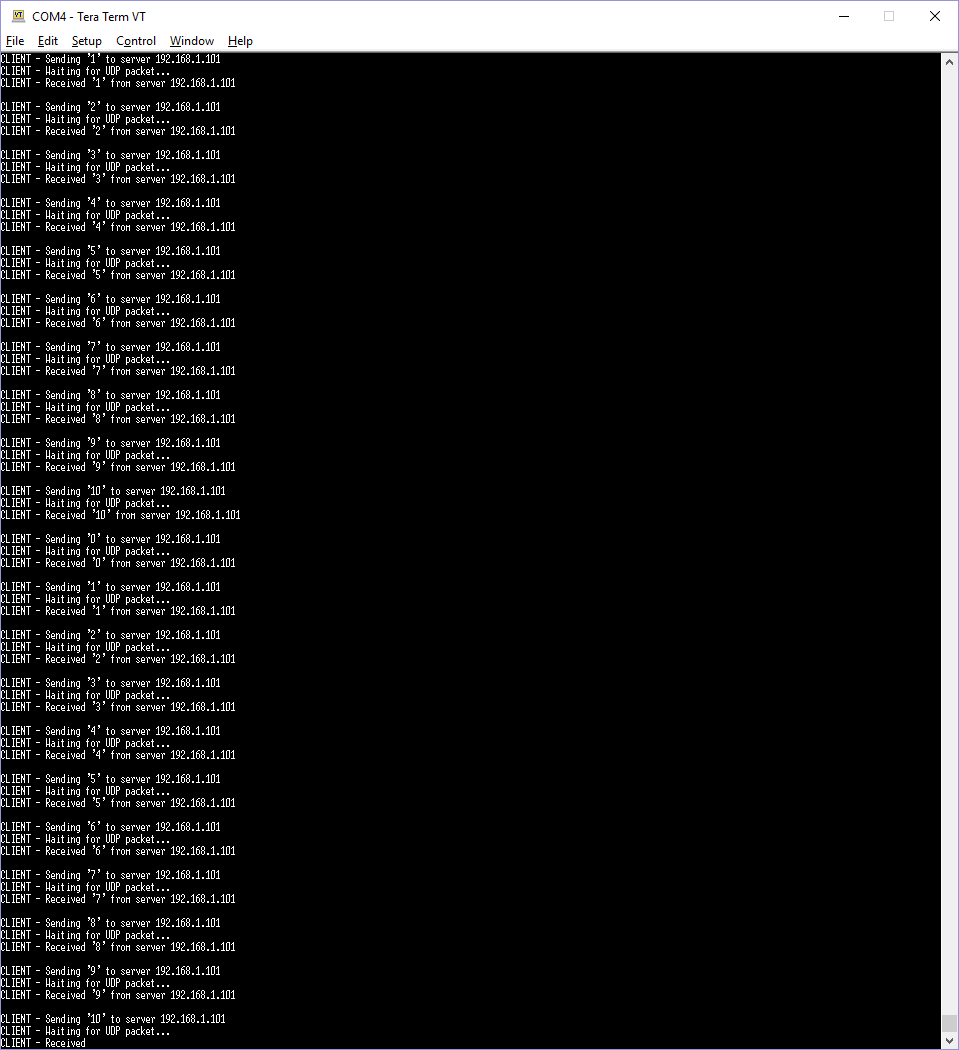
\includegraphics[width=\textwidth]{Client}
					\caption{shows the tera term output from the client application}
					\label{img:ex1-client}
				\end{figure}
				\begin{figure}
					\centering
					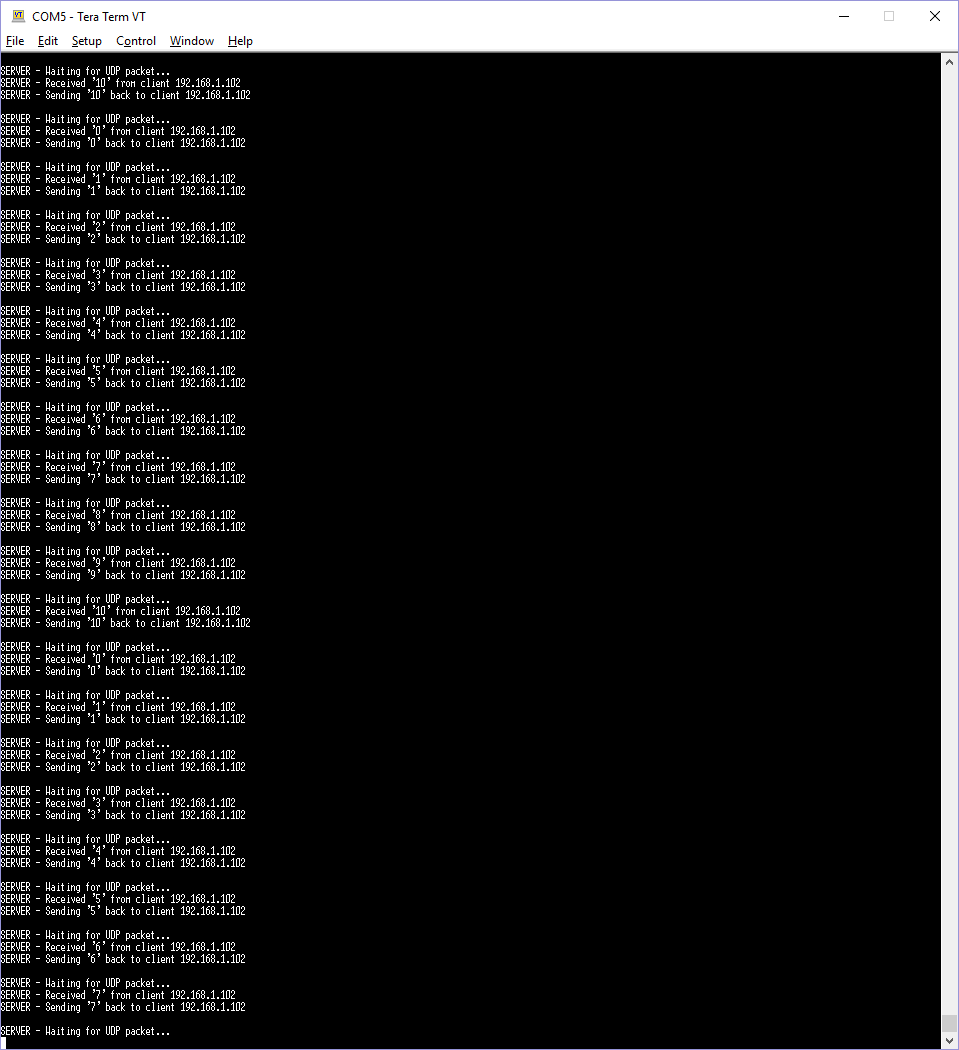
\includegraphics[width=\textwidth]{Server}
					\caption{shows the tera term output from the server application}
					\label{img:ex1-server}
				\end{figure}
			}
			\subsection{Exercise 2}
			{
				This involved me attempting to send the accelerometer data from one board to the other and vice versa. However the first problem I hit was that the sockets library we are using does not support the sending of floats. which is not too surprising however after this I attempted to convert the float into a char array so I could send that over the Ethernet cable however whenever I attempted to read that char array I had weird values in it. Unfortunately I ran out of time due to the problem earlier meaning that I was unable to get this working. The code for this can be found in \cref{appendix:ex2-Client} and \cref{appendix:ex2-Server} also \cref{img:ex2-client} and  \cref{img:ex2-server} shows the gibberish output I was talking about.
				\begin{figure}
					\centering
					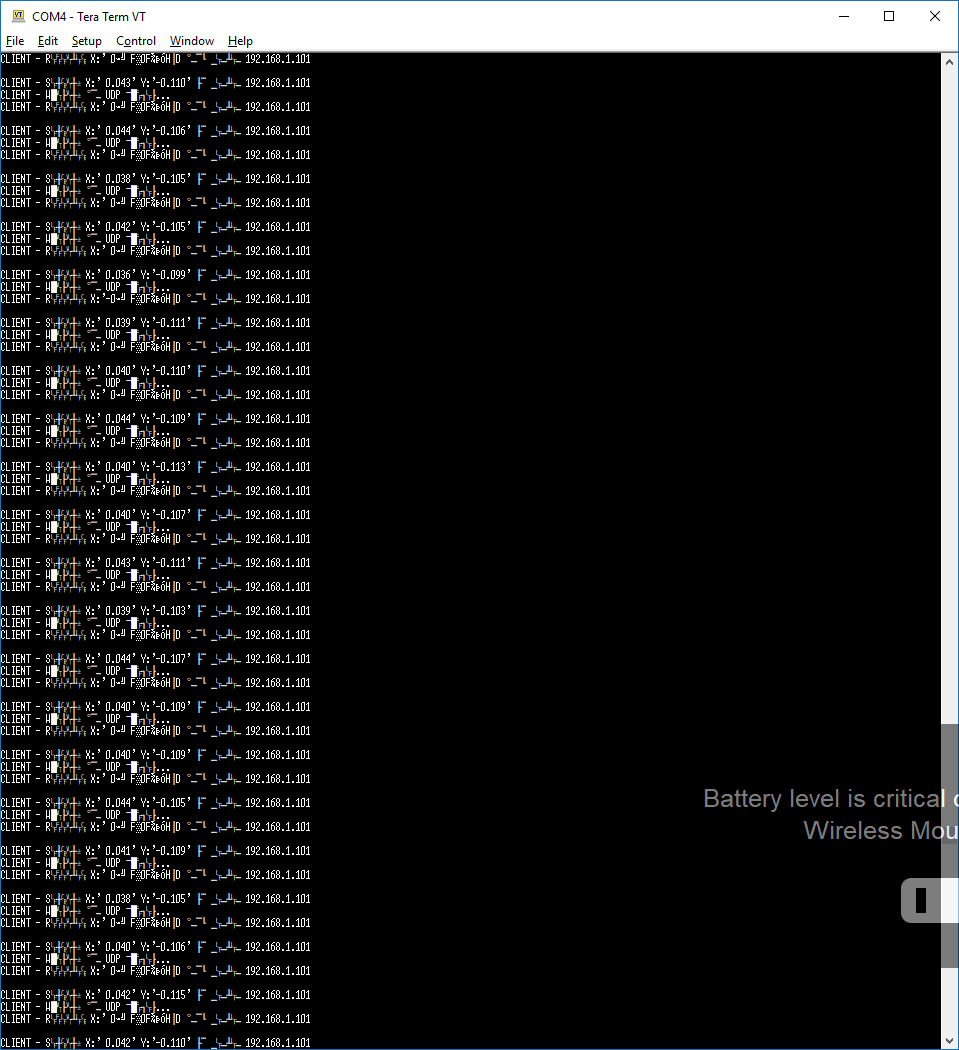
\includegraphics[width=\textwidth]{ClientAcceleratorData}
					\caption{shows the tera term output from the client application}
					\label{img:ex2-client}
				\end{figure}
				\begin{figure}
					\centering
					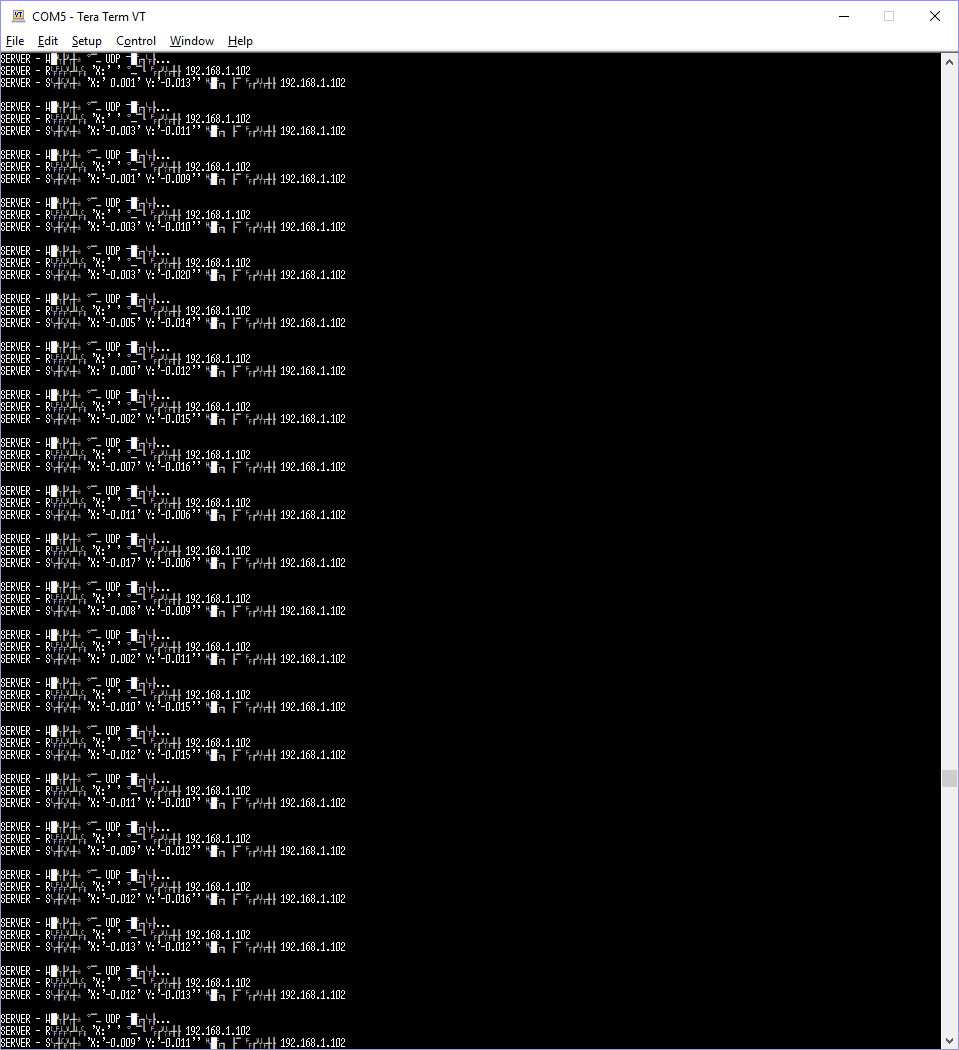
\includegraphics[width=\textwidth]{ServerAcceleratorData}
					\caption{shows the tera term output from the server application}
					\label{img:ex2-server}
				\end{figure}
			}
		}
		\subsection{Connecting to IBMs Internet of Things}
		{
			I had to use the program at \url{https://os.mbed.com/users/steveshun/code/IoTClientEthernet/} to allow me to manually set the MAC address of the board allowing me to run it over the University's network. After that it was quite simple to work and I got the image shown in \cref{img:IBMIoT} which shows the values of the sensors on the board. 
			\begin{figure}
				\centering
				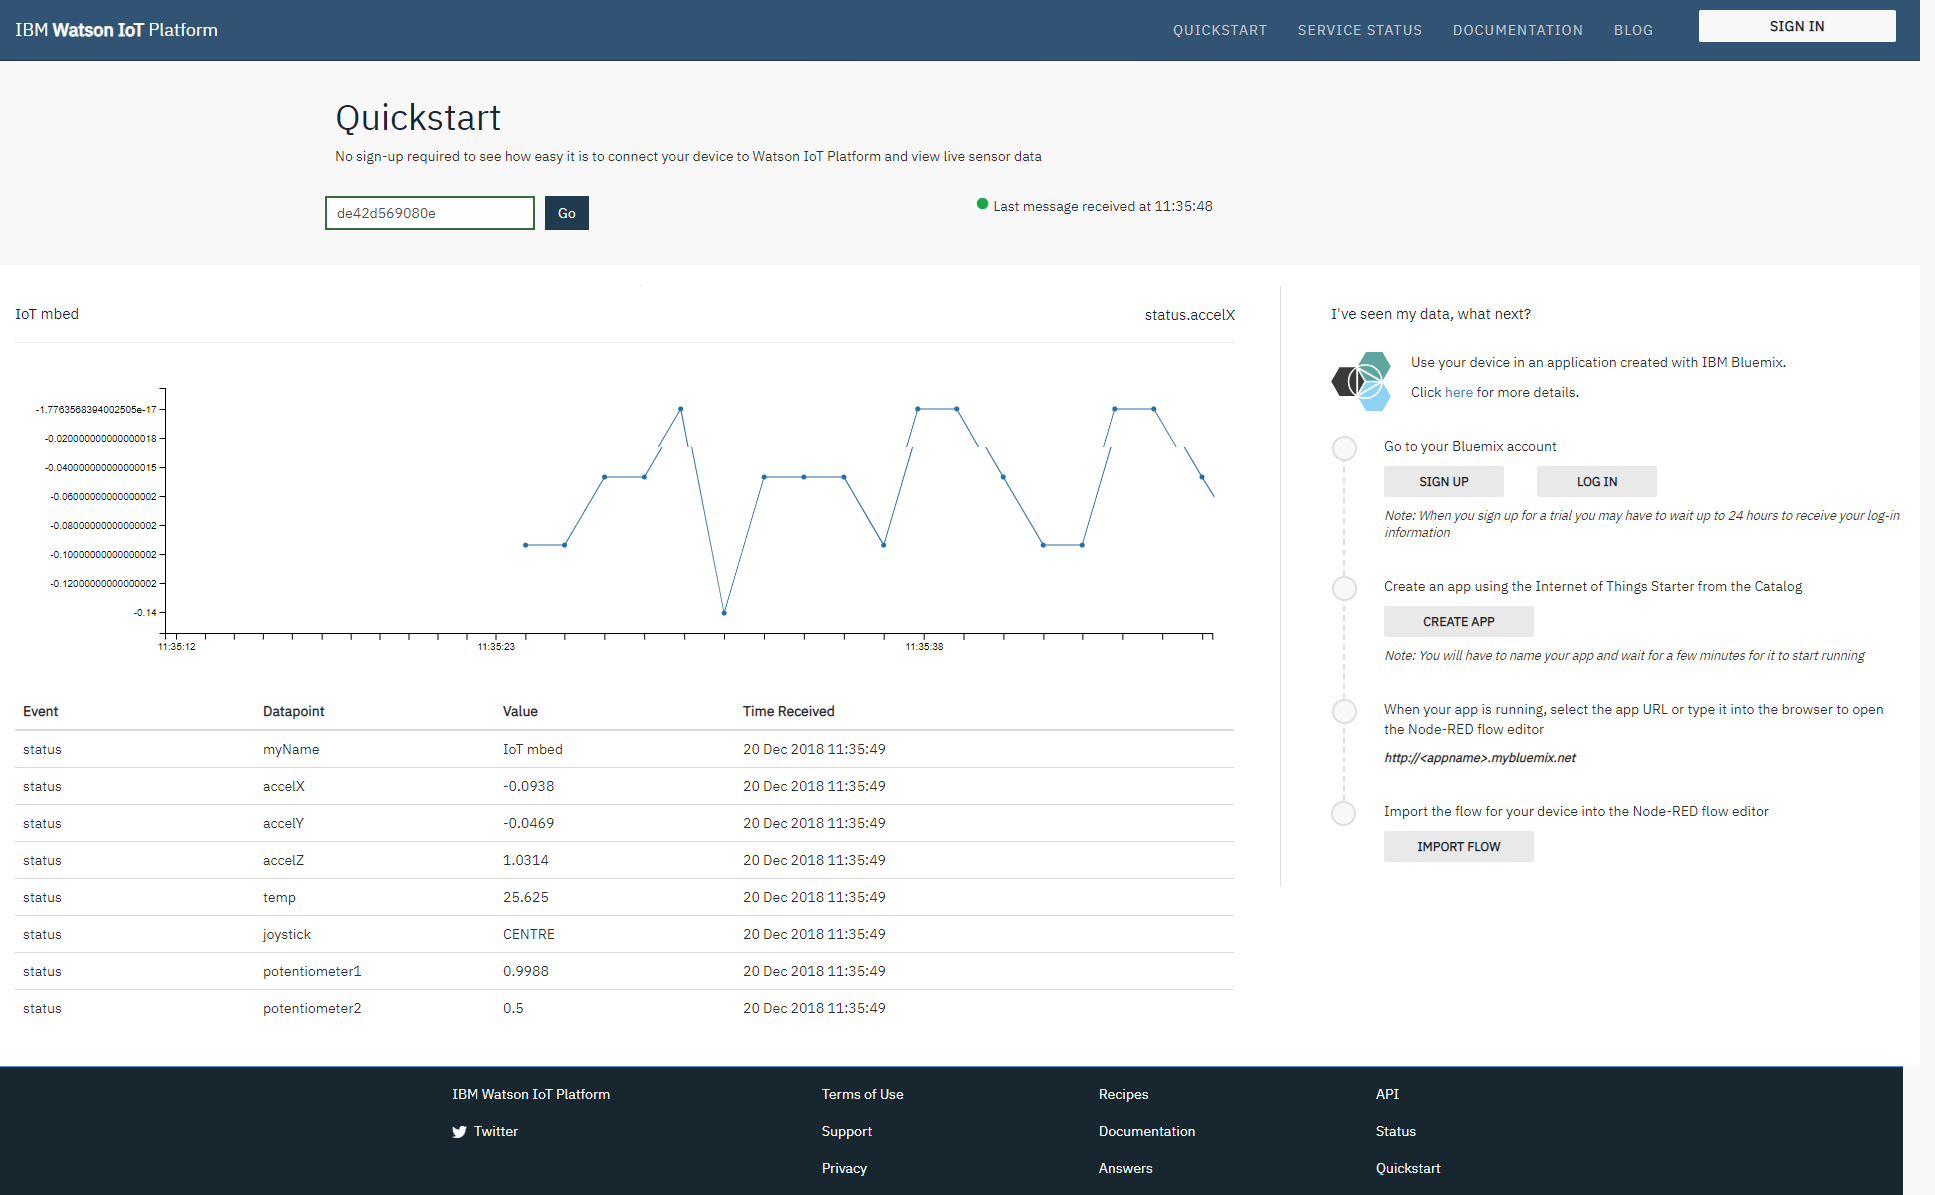
\includegraphics[width=\textwidth]{IBMIoT}
				\caption{shows the display from the IBM IoT Application which describles the state of the board}
				\label{img:IBMIoT}
			\end{figure}
		}
	}
	\section{Conclusion}
	{
		In conclusion, this was a useful exercise on using Ethernet communications and then how to use and set-up the device as an Internet of things devices. This served as a useful start for the project I plan on completing over the winter.
	}
	
	\newpage
	\begin{appendices}
	\label{Appendix:start}
	\section{Lab Exercise 1}
	{
		\subsection{Part 1}
		{
			\label{appendix:ex1-1}
			\lstinputlisting[language=c++]{CodeListings/Ex1/mainPart1.cpp}
		}
		\subsection{Part 2}
		{
			\label{appendix:ex1-2}
			\lstinputlisting[language=c++]{CodeListings/Ex1/mainPart2.cpp}
		}
		\subsection{Part 3}
		{
			\label{appendix:ex1-3}
			\lstinputlisting[language=c++]{CodeListings/Ex1/mainPart3.cpp}
		}
	}
	\section{Lab Exercise 2}
	{
		\label{appendix:ex2}
		\subsection{Part 1 - Master Program}
		{
			\label{appendix:ex2-1}
			\lstinputlisting[language=c++]{CodeListings/Ex2/main-master.cpp}
		}
		\subsection{Part 2 - Slave Program}
		{
			\label{appendix:ex2-2}
			\lstinputlisting[language=c++]{CodeListings/Ex2/main-slave.cpp}
		}
	}

\end{appendices}
	\printbibliography[heading=bibintoc,title=References]
\end{document}
